\documentclass[10pt,a4paper]{report}
\usepackage[utf8]{inputenc}
\usepackage{amsmath}
\usepackage{amsfonts}
\usepackage{amssymb}
\usepackage{graphicx}
\usepackage{bm}
\usepackage{gensymb}
\usepackage[left=2cm,right=2cm,top=2cm,bottom=2cm]{geometry}
\setlength\parindent{0pt}
\usepackage{float}
\graphicspath{{./images/}}
\begin{document}


\textbf{Core Project 1.2: Ordinary Differential Equations}
\thispagestyle{empty}

\newpage


\subsection*{Programming task}

The functions $eulersolve, LFsolve, RK4solveOLD$ each take inputs the function $f$, $x_0, y_0$, h and n, and output arrays X and Y. They can be found on page 16. The elements of Y are the numerical solution for the corresponding value of X. The LF method takes the first step via the euler method. \\

Testing our program works as intended, using $ProgramTest.m$, found on page 16: 

\begin{figure}[H]
\centering
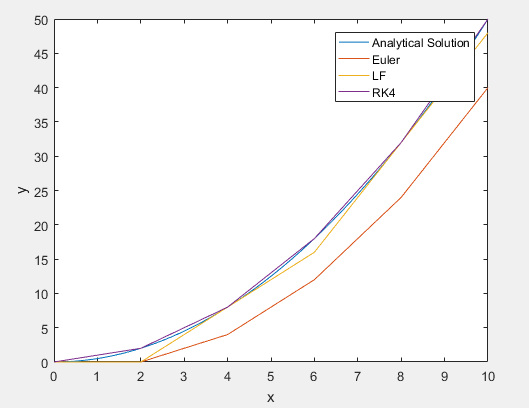
\includegraphics[scale=0.8]{test}
\caption{A plot of our numerical methods solutions with $h=2$ $x_0=y_0=0$ $f(x)=x$}
\end{figure}

\begin{figure}[H]
\centering
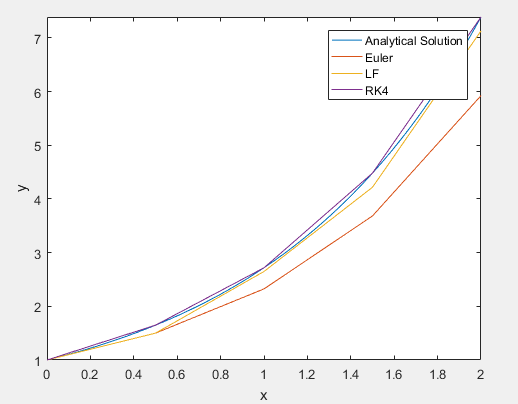
\includegraphics[scale=0.8]{test12}
\caption{A plot of our numerical methods solutions with $h=0.5$ $x_0=0$, $y_0=1$, $f(x)=e^x$}
\end{figure}

These are close enough to the analytical solution to verify our functions are working as intended.

\subsection*{Question 1}
We use the function $q1$, shown on page 17. To verify the exponential relationship of the magnitude of global error with x we plot a graph of x against $log(|E_n|)$ and see it is near straight (excluding the 0 error at 0). We use an inbuilt MATLAB function to approximate this to a polynomial of degree 1 and take the gradient. \\\

For $h=0.4$ we have the following. Figure 3 validates the exponential relationship, with a corresponding $\gamma\approx 3.13$

\begin{verbatim}
>> [X,Y_LF,Y,E] = q1(0.4)
\end{verbatim}



\begin{minipage}[b]{0.45\linewidth}
\centering
\begin{table}[H]
\begin{tabular}{|l|l|l|l|}
\hline
$X_n$ & $Y_n$      & $y(x_n)$  & $E_n$      \\ \hline
0    & 0.00E+00  & 0.00E+00 & 0.00E+00  \\ \hline
0.4  & 1.20E+00  & 4.68E-01 & 7.32E-01  \\ \hline
0.8  & -2.23E+00 & 4.09E-01 & -2.64E+00 \\ \hline
1.2  & 9.42E+00  & 2.93E-01 & 9.13E+00  \\ \hline
1.6  & -3.16E+01 & 2.00E-01 & -3.18E+01 \\ \hline
2    & 1.11E+02  & 1.35E-01 & 1.11E+02  \\ \hline
2.4  & -3.87E+02 & 9.07E-02 & -3.87E+02 \\ \hline
2.8  & 1.35E+03  & 6.08E-02 & 1.35E+03  \\ \hline
3.2  & -4.71E+03 & 4.08E-02 & -4.71E+03 \\ \hline
3.6  & 1.64E+04  & 2.73E-02 & 1.64E+04  \\ \hline
4    & -5.72E+04 & 1.83E-02 & -5.72E+04 \\ \hline
4.4  & 2.00E+05  & 1.23E-02 & 2.00E+05  \\ \hline
4.8  & -6.96E+05 & 8.23E-03 & -6.96E+05 \\ \hline
5.2  & 2.43E+06  & 5.52E-03 & 2.43E+06  \\ \hline
5.6  & -8.46E+06 & 3.70E-03 & -8.46E+06 \\ \hline
6    & 2.95E+07  & 2.48E-03 & 2.95E+07  \\ \hline
6.4  & -1.03E+08 & 1.66E-03 & -1.03E+08 \\ \hline
6.8  & 3.59E+08  & 1.11E-03 & 3.59E+08  \\ \hline
7.2  & -1.25E+09 & 7.47E-04 & -1.25E+09 \\ \hline
7.6  & 4.36E+09  & 5.00E-04 & 4.36E+09  \\ \hline
8    & -1.52E+10 & 3.35E-04 & -1.52E+10 \\ \hline
8.4  & 5.30E+10  & 2.25E-04 & 5.30E+10  \\ \hline
8.8  & -1.85E+11 & 1.51E-04 & -1.85E+11 \\ \hline
9.2  & 6.44E+11  & 1.01E-04 & 6.44E+11  \\ \hline
9.6  & -2.25E+12 & 6.77E-05 & -2.25E+12 \\ \hline
10   & 7.83E+12  & 4.54E-05 & 7.83E+12  \\ \hline
\end{tabular}
\caption{Output with $h=0.4$}
\end{table}
\end{minipage}
\hspace{0.5cm}
\begin{minipage}[b]{0.45\linewidth}
\begin{figure}[H]
\centering
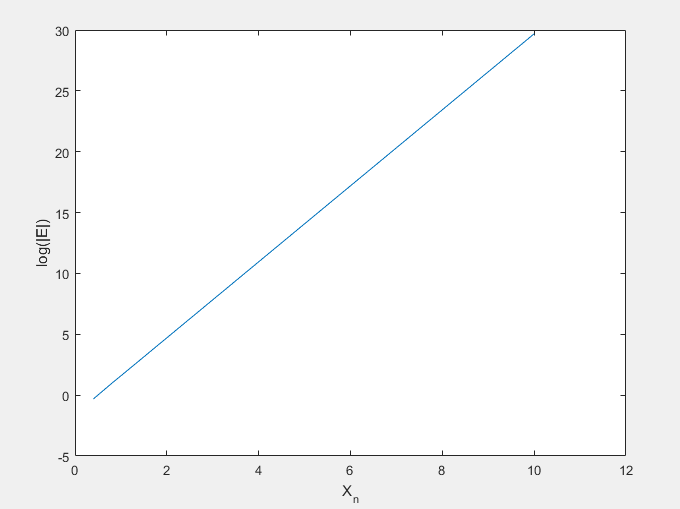
\includegraphics[width=\textwidth]{q1n25}
\caption{A plot of $log(|E_n|)$ against $X_n$}
\end{figure}
\vspace{2.5cm}
\end{minipage}

\vspace{0.5cm}
For the remaining h, we omit including the straight line $log(|E_n|)$ and simply give the $\gamma$. We also omit some data from the table. Note due to the selection of  even data points the oscillation in error is not displayed, but is still present.\\

For h=0.2 we have $\gamma\approx 3.66$, for h=0.1 we have $\gamma\approx 3.90$ and for $h=0.05$ we have $\gamma\approx3.97$.

\begin{minipage}[b]{0.45\linewidth}
\centering

\begin{table}[H]
\begin{tabular}{|l|l|l|l|}
\hline
$X_n$ & $Y_n$      & $y(x_n)$  & $E_n$      \\ \hline
0    & 0.00E+00  & 0.00E+00 & 0.00E+00  \\ \hline
0.4  & 2.25E-02  & 4.68E-01 & -4.46E-01 \\ \hline
0.8  & -1.51E+00 & 4.09E-01 & -1.92E+00 \\ \hline
1.2  & -7.98E+00 & 2.93E-01 & -8.27E+00 \\ \hline
1.6  & -3.56E+01 & 2.00E-01 & -3.58E+01 \\ \hline
2    & -1.55E+02 & 1.35E-01 & -1.55E+02 \\ \hline
2.4  & -6.71E+02 & 9.07E-02 & -6.71E+02 \\ \hline
2.8  & -2.90E+03 & 6.08E-02 & -2.90E+03 \\ \hline
3.2  & -1.26E+04 & 4.08E-02 & -1.26E+04 \\ \hline
3.6  & -5.44E+04 & 2.73E-02 & -5.44E+04 \\ \hline
4    & -2.36E+05 & 1.83E-02 & -2.36E+05 \\ \hline
4.4  & -1.02E+06 & 1.23E-02 & -1.02E+06 \\ \hline
4.8  & -4.42E+06 & 8.23E-03 & -4.42E+06 \\ \hline
5.2  & -1.91E+07 & 5.52E-03 & -1.91E+07 \\ \hline
5.6  & -8.28E+07 & 3.70E-03 & -8.28E+07 \\ \hline
6    & -3.58E+08 & 2.48E-03 & -3.58E+08 \\ \hline
6.4  & -1.55E+09 & 1.66E-03 & -1.55E+09 \\ \hline
6.8  & -6.71E+09 & 1.11E-03 & -6.71E+09 \\ \hline
7.2  & -2.91E+10 & 7.47E-04 & -2.91E+10 \\ \hline
7.6  & -1.26E+11 & 5.00E-04 & -1.26E+11 \\ \hline
8    & -5.45E+11 & 3.35E-04 & -5.45E+11 \\ \hline
8.4  & -2.36E+12 & 2.25E-04 & -2.36E+12 \\ \hline
8.8  & -1.02E+13 & 1.51E-04 & -1.02E+13 \\ \hline
9.2  & -4.42E+13 & 1.01E-04 & -4.42E+13 \\ \hline
9.6  & -1.91E+14 & 6.77E-05 & -1.91E+14 \\ \hline
10   & -8.28E+14 & 4.54E-05 & -8.28E+14 \\ \hline
\end{tabular}
\caption{Output with $h=0.2$}
\end{table}

\end{minipage}
\hspace{0.5cm}
\begin{minipage}[b]{0.45\linewidth}



\begin{table}[H]
\centering
\begin{tabular}{|l|l|l|l|}
\hline
$X_n$ & $Y_n$      & $y(x_n)$  & $E_n$      \\ \hline
0    & 0.00E+00  & 0.00E+00 & 0.00E+00  \\ \hline
0.4  & 3.08E-01  & 4.68E-01 & -1.60E-01 \\ \hline
0.8  & -3.51E-01 & 4.09E-01 & -7.60E-01 \\ \hline
1.2  & -3.31E+00 & 2.93E-01 & -3.61E+00 \\ \hline
1.6  & -1.70E+01 & 2.00E-01 & -1.72E+01 \\ \hline
2    & -8.16E+01 & 1.35E-01 & -8.17E+01 \\ \hline
2.4  & -3.89E+02 & 9.07E-02 & -3.89E+02 \\ \hline
2.8  & -1.85E+03 & 6.08E-02 & -1.85E+03 \\ \hline
3.2  & -8.81E+03 & 4.08E-02 & -8.81E+03 \\ \hline
3.6  & -4.19E+04 & 2.73E-02 & -4.19E+04 \\ \hline
4    & -2.00E+05 & 1.83E-02 & -2.00E+05 \\ \hline
4.4  & -9.50E+05 & 1.23E-02 & -9.50E+05 \\ \hline
4.8  & -4.52E+06 & 8.23E-03 & -4.52E+06 \\ \hline
5.2  & -2.15E+07 & 5.52E-03 & -2.15E+07 \\ \hline
5.6  & -1.02E+08 & 3.70E-03 & -1.02E+08 \\ \hline
6    & -4.87E+08 & 2.48E-03 & -4.87E+08 \\ \hline
6.4  & -2.32E+09 & 1.66E-03 & -2.32E+09 \\ \hline
6.8  & -1.10E+10 & 1.11E-03 & -1.10E+10 \\ \hline
7.2  & -5.26E+10 & 7.47E-04 & -5.26E+10 \\ \hline
7.6  & -2.50E+11 & 5.00E-04 & -2.50E+11 \\ \hline
8    & -1.19E+12 & 3.35E-04 & -1.19E+12 \\ \hline
8.4  & -5.67E+12 & 2.25E-04 & -5.67E+12 \\ \hline
8.8  & -2.70E+13 & 1.51E-04 & -2.70E+13 \\ \hline
9.2  & -1.28E+14 & 1.01E-04 & -1.28E+14 \\ \hline
9.6  & -6.11E+14 & 6.77E-05 & -6.11E+14 \\ \hline
10   & -2.91E+15 & 4.54E-05 & -2.91E+15 \\ \hline
\end{tabular}
\caption{Output with $h=0.1$}
\end{table}

\end{minipage}


\begin{table}[H]
\centering
\begin{tabular}{|l|l|l|l|}
\hline
$X_n$ & $Y_n$      & $y(x_n)$  & $E_n$      \\ \hline
0        & 0.00E+00  & 0.00E+00 & 0.00E+00  \\ \hline
0.4      & 4.24E-01  & 4.68E-01 & -4.48E-02 \\ \hline
0.8      & 1.90E-01  & 4.09E-01 & -2.19E-01 \\ \hline
1.2      & -7.78E-01 & 2.93E-01 & -1.07E+00 \\ \hline
1.6      & -5.05E+00 & 2.00E-01 & -5.25E+00 \\ \hline
2        & -2.56E+01 & 1.35E-01 & -2.57E+01 \\ \hline
2.4      & -1.26E+02 & 9.07E-02 & -1.26E+02 \\ \hline
2.8      & -6.18E+02 & 6.08E-02 & -6.18E+02 \\ \hline
3.2      & -3.03E+03 & 4.08E-02 & -3.03E+03 \\ \hline
3.6      & -1.49E+04 & 2.73E-02 & -1.49E+04 \\ \hline
4        & -7.28E+04 & 1.83E-02 & -7.28E+04 \\ \hline
4.4      & -3.57E+05 & 1.23E-02 & -3.57E+05 \\ \hline
4.8      & -1.75E+06 & 8.23E-03 & -1.75E+06 \\ \hline
5.2      & -8.57E+06 & 5.52E-03 & -8.57E+06 \\ \hline
5.6      & -4.20E+07 & 3.70E-03 & -4.20E+07 \\ \hline
6        & -2.06E+08 & 2.48E-03 & -2.06E+08 \\ \hline
6.4      & -1.01E+09 & 1.66E-03 & -1.01E+09 \\ \hline
6.8 & -4.95E+09 & 1.11E-03 & -4.95E+09 \\ \hline
7.2 & -2.42E+10 & 7.47E-04 & -2.42E+10 \\ \hline
7.6 & -1.19E+11 & 5.00E-04 & -1.19E+11 \\ \hline
8.0 & -5.83E+11 & 3.35E-04 & -5.83E+11 \\ \hline
8.4 & -2.86E+12 & 2.25E-04 & -2.86E+12 \\ \hline
8.8 & -1.40E+13 & 1.51E-04 & -1.40E+13 \\ \hline
9.2 & -6.86E+13 & 1.01E-04 & -6.86E+13 \\ \hline
9.6 & -3.36E+14 & 6.77E-05 & -3.36E+14 \\ \hline
10 & -1.65E+15 & 4.54E-05 & -1.65E+15 \\ \hline
\end{tabular}
\caption{Output with $h=0.05$}
\end{table}

In general, reducing h seems to increase the growth rate, and it would appear $\gamma$ tends to some limit $\approx 4$ as h tends to 0. Thus, for sufficiently small h, decreasing h further reduces magnitude of error as the growth rate increase slows.	



\subsection*{Question 2}

i) We have the difference equation

\begin{equation*}
Y_{n+1}+8hY_n-Y_{n-1}=6he^{-hn}
\end{equation*}

which, we know from IA Differential Equations can be solved in a similar fashion to ODEs. We first assume a complementary function of form $k^n$. Our auxiliary equation becomes

\begin{equation*}
k^2+8hk-1=0
\end{equation*}

leading to solutions 

\begin{equation*}
k_\pm=-4h\pm\sqrt{16h^2+1}
\end{equation*}

For a particular integral we try a form $Y_p=Ce^{-hn}$ and find

\begin{equation*}
C=\frac{6h}{e^{-h}+8h-e^h}
\end{equation*}

Hence have a solution

\begin{equation*}
Y_n=A(k_+)^n + B(k_-)^n +\frac{6he^{-hn}}{e^{-h}+8h-e^h}
\end{equation*}

Solving for A and B with the initial conditions we find

\begin{equation*}
A=\frac{-3h(e^{-h} + 8h - e^h)+6h\sqrt{16h^2+1}+6he^{-h}}{(e^{-h} + 8h - e^h)(-2\sqrt{16h^2+1})}
\end{equation*}
\begin{equation*}
B=\frac{3h(e^{-h} + 8h - e^h)+6h\sqrt{16h^2+1}-6he^{-h}}{(e^{-h} + 8h - e^h)(-2\sqrt{16h^2+1})}
\end{equation*}

ii) We see the reason for the instability here. We have for positive h the term $k_-$ being greater than 1 in magnitude and negative. Thus the $(k_-)^n$ term oscillates and becomes very large in magnitude with all other terms quickly tending to 0 as n increases.\\

iii) Consider the limit $h \rightarrow 0$, $n \rightarrow \infty$ with $x_n=nh$ fixed.\\ \vspace{0.2cm}

By L'hopitals rule, $\frac{6h}{(e^{-h} + 8h - e^h)}$ tends to 1 as $h \rightarrow 0$, so $\frac{6he^{-hn}}{e^{-h}+8h-e^h} \rightarrow e^{-x_n}$\\

We have

\begin{equation*}
A=
\frac{-3h}{-2\sqrt{16h^2+1}} + 
\frac{6h}{-2(e^{-h} + 8h - e^h)} +
\frac{6h}{(e^{-h} + 8h - e^h)}
\frac{e^-h}{-2\sqrt{16h^2+1}}
\end{equation*}

where the first term $\rightarrow 0$, the second and third $\rightarrow -\frac{1}{2}$ and thus $A\rightarrow -1$. %and since $(k_+)^n \rightarrow 0$ (as $k_+ < 1$) the whole first term $A(k_+)^n \rightarrow 0$

\begin{align*}
(-4h+\sqrt{16h^2+1})^n = (-\frac{4x}{n}+\sqrt{\frac{16x^2}{n^2}+1})^n= (\frac{16x^2}{n^2}+1)^{n/2}(1-\frac{4x}{n}(16\frac{x^2}{n^2}+1)^{-1/2})^n
\end{align*}

%For any $\varepsilon>0$ and $n>N$ for some sufficiently large N

%\begin{align*}
%(1-\frac{4x}{n}) \leq (1-\frac{4x}{n}(16\frac{x^2}{n^2}+1)^{-1/2}) \leq (1-\frac{4x}{n+%%%\varepsilon})
%\end{align*}

%and

%\begin{equation*}
%1 \leq \frac{16x^2}{n^2}+1 \leq 1+\varepsilon
%\end{equation*}

%And thus taking the n'th and n/2th powers respectively,with $\varepsilon\rightarrow 0$ shows, %as $n\rightarrow\infty$

%\begin{align*}
%(1-\frac{4x}{n}(16\frac{x^2}{n^2}+1)^{-1/2})^n &\rightarrow e^{-4x}\\
%(\frac{16x^2}{n^2}+1)^{n/2} &\rightarrow 1
%\end{align*}
Now let

\begin{align*}
z_n &= (1-\frac{4x}{n}(16\frac{x^2}{n^2}+1)^{-1/2})^n \\
\Rightarrow log(z_n)&=nlog(1-\frac{4x}{n}(16\frac{x^2}{n^2}+1)^{-1/2})
\end{align*}

and taylor expanding the log (which we can do as $|\frac{4x}{n}(16\frac{x^2}{n^2}+1)^{-1/2})|<1$)`

\begin{align*}
log(z_n) &= n(-\frac{4x}{n}(16\frac{x^2}{n^2}+1)^{-1/2}-\frac{16x^2}{n^2}(16\frac{x^2}{n^2}+1)^{-1}+o(\frac{16x^2}{n^2}(16\frac{x^2}{n^2}+1)^{-1}))\\
&=-4x(16\frac{x^2}{n^2}+1)^{-1/2}-	\frac{16x^2}{n}(16\frac{x^2}{n^2}+1)^{-1/2}+o(1) \rightarrow -4x
\end{align*}

so as $n\rightarrow\infty$, $z_n\rightarrow e^{-4x}$.  Now, let

\begin{align*}
q_n &= (1+\frac{16x^2}{n^2})^{n/2}\\
\Rightarrow log(q_n)&=\frac{n}{2}log(1+\frac{16x^2}{n^2})\\
\Rightarrow log(q_n)&=\frac{16x^2}{n}+o(\frac{1}{n}) \rightarrow 0\\
\Rightarrow q_n \rightarrow 1
\end{align*}

hence the 'A' term $\rightarrow -e^{-4x}$. By a similar method to above, $B\rightarrow 0 $ and $|(k_-)^n| \rightarrow e^{4x}$ hence the term goes to 0. Hence, 

\begin{equation*}
Y_n \rightarrow e^{-x_n} - e^{-4x_n}
\end{equation*}

This however does not mean the instability can necessarily be suppressed with small h. Looking at the expression for $Y_n$, no matter how small h is, we will still have instability as n (and thus x) grows. This makes sense, since we have shown pointwise convergence, but not uniform convergence. Instability is a global and not a local property, and hence we require uniform convergence to suppress it.

\newpage


\subsection*{Question 3}

The script $q3.m$, shown on page 17, uses the previously written functions to produce the data and graph

\begin{verbatim}

>> q3

\end{verbatim}


\begin{figure}[ht]
\begin{minipage}[b]{0.3\linewidth}


\begin{table}[H]
\centering
\begin{tabular}{|l|l|l|}
\hline


$X_n$ & $Y_n$ Euler & $Y_n$ RK4 \\ \hline
0    & 0.0000     & 0.0000   \\ \hline
0.4  & 1.2000     & 0.4059   \\ \hline
0.8  & 0.0844     & 0.3818   \\ \hline
1.2  & 0.4886     & 0.2856   \\ \hline
1.6  & 0.0683     & 0.1995   \\ \hline
2    & 0.2013     & 0.1359   \\ \hline
2.4  & 0.0416     & 0.0917   \\ \hline
2.8  & 0.0839     & 0.0616   \\ \hline
3.2  & 0.0226     & 0.0413   \\ \hline
3.6  & 0.0353     & 0.0277   \\ \hline
4    & 0.0116     & 0.0186   \\ \hline
\end{tabular}


\caption{Output with h=0.4}
\end{table}

\vspace{2cm}
\end{minipage}
\hspace{0.5cm}
\begin{minipage}[b]{0.6\linewidth}
\centering
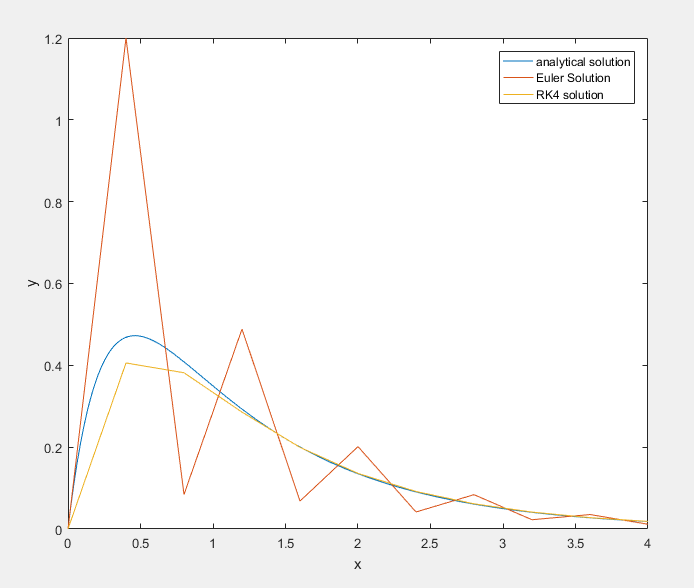
\includegraphics[width=\textwidth]{q3}
\caption{A graph showing numerical solutions and the analytical one for h=0.4}

\end{minipage}
\end{figure}

\subsection*{Question 4}

Again, we reuse our previous functions; the script $q4.m$, shown on page 18 produces the following output.

\begin{verbatim}

>> q4

\end{verbatim}


\begin{figure}[ht]

\begin{minipage}[b]{0.4\linewidth}
\centering


\begin{table}[H]

\begin{tabular}{|l|l|l|l|}
\hline
k  & $E_n$ Euler & $E_n$ LF     & $E_n$ RK4    \\ \hline
0  & 7.32E-01   & 7.32E-01  & -6.26E-02 \\ \hline
1  & 1.43E-01   & -4.46E-01 & -1.92E-03 \\ \hline
2  & 6.37E-02   & -1.60E-01 & -8.42E-05 \\ \hline
3  & 3.00E-02   & -4.48E-02 & -4.41E-06 \\ \hline
4  & 1.46E-02   & -1.15E-02 & -2.53E-07 \\ \hline
5  & 7.20E-03   & -2.91E-03 & -1.51E-08 \\ \hline
6  & 3.57E-03   & -7.28E-04 & -9.24E-10 \\ \hline
7  & 1.78E-03   & -1.82E-04 & -5.71E-11 \\ \hline
8  & 8.89E-04   & -4.55E-05 & -3.55E-12 \\ \hline
9  & 4.44E-04   & -1.14E-05 & -2.22E-13 \\ \hline
10 & 2.22E-04   & -2.85E-06 & -1.37E-14 \\ \hline
11 & 1.11E-04   & -7.12E-07 & 2.11E-15  \\ \hline
12 & 5.55E-05   & -1.78E-07 & -8.88E-16 \\ \hline
13 & 2.77E-05   & -4.45E-08 & -1.23E-14 \\ \hline
14 & 1.39E-05   & -1.11E-08 & 5.00E-15  \\ \hline
15 & 6.93E-06   & -2.78E-09 & 4.30E-14  \\ \hline
\end{tabular}

\caption{Output of q4.m}

\vspace{0.5cm}

\end{table}

\end{minipage}
\hspace{0.5cm}
\begin{minipage}[b]{0.6\linewidth}
\centering
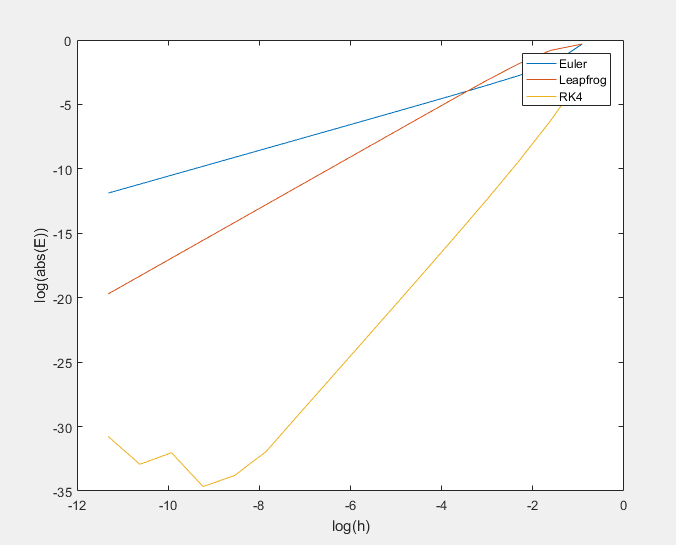
\includegraphics[width=\textwidth]{q4}
\caption{A graph of $log|E_n|$ against $logh$  at $x_n=0.4$ for each of the three numerical methods}

\end{minipage}
\end{figure}

\newpage

The given information tells us about the behaviour of local truncation error $e_n$ as $h \rightarrow 0$, but here we are looking at global error at $x_n=0.4$. The global error is the effect of all the local error's up to time $x_n=0.4$, of which there are $\frac{0.4}{h}$. If the local error is $O(h^m)$ this implies the global error should be $O(h^{m-1})$, and hence the gradient of the graph of figure 5 should be $m-1$. We can see this is  true, with the euler gradient being $\approx 1$, the leapfrog gradient $\approx 2$, and the RK4 gradient(atleast while linear) being $\approx 4$, confirming the theoretical accuracy. The fluctuation from linear for very small h in the RK4 method can be attributed to machine error, as we are very close to MATLAB's 'double' precision in the errors here.


\newpage

\subsection*{Question 5}

We have the ODE

\begin{equation*}
\frac{d^2y}{dt^2} + \gamma\frac{dy}{dt}+\Omega^2y=asin(\omega t)
\end{equation*}

The auxiliary equation gives solutions 

\begin{equation*}
\lambda = \frac{- \gamma \pm i \sqrt{4 \Omega ^2 - \gamma ^2}}{2}
\end{equation*}

leading to a complementary function 

\begin{equation*}
y_c=e^{-\frac{\gamma t}{2}}(Acos(\frac{\sqrt{4 \Omega ^2 - \gamma ^2}}{2}t)+Bsin(\frac{\sqrt{4 \Omega ^2 - \gamma ^2}}{2}t))
\end{equation*}

for arbitrary A and B. Note $y_c \rightarrow 0$ as $t\rightarrow\infty$ for all A,B. We look for a particular integral of form

\begin{equation*}
y_p=Csin(\omega t) + Dcos(\omega t)
\end{equation*}

and find

\begin{equation*}
C=-\frac{(\omega^2-\Omega^2)a}{\gamma^2\omega^2+(w^2-\Omega^2)^2}
\quad
D=-\frac{\omega\gamma a}{\gamma^2\omega^2+(w^2-\Omega^2)^2}
\end{equation*}

Then $y_p$ can be put in the required form $ A_s sin(\omega t - \varphi_s)$ with

\begin{equation*}
A_s = \frac{a}{\sqrt{\gamma^2\omega^2+(\omega^2-\Omega^2)^2}}
\quad
tan(\phi _s) = \frac{\omega\gamma}{\Omega^2-\omega^2}
\end{equation*}

We are done since $y=y_c+y_p\rightarrow y_p$

\subsection*{Programming Task}

We modify our previous RK4 function to allow it to take a vector valued function $f$, so it can solve a system of coupled first order ODEs. To test it works, we consider the system

\begin{equation*}
y''+y=0 \quad y(0)=1, \quad y'(0)=0
\end{equation*}

with solution $y=cosx$. Note we can write the system as 

\begin{equation*}
\bm{y}=[y_1, y_2]:=[y, y'] \quad \bm{y}'=[y_2,-y_1]=f(x,\bm{y})
\end{equation*}

Solving this using our new RK4 function, using the script $ProgramTest2.m$, found on page 19, we get figure 5. This is sufficiently near to the analytical solution to verify our new function does work as intended.

\begin{figure}[H]
\centering
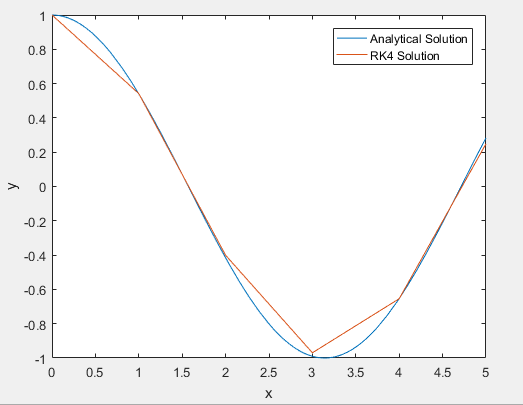
\includegraphics[scale=0.8]{test2}
\caption{A plot of our RK4 solution against the analytical solution with h=1}
\end{figure}

\subsection*{Question 6}

We take the above general form and calculate the values of constants A and B to fit the initial conditions. We use the slightly more complicated $y_p$ involving C and D to avoid dealing with an arctan, giving

\begin{multline*}
y = e^{-\frac{\gamma t}{2}}\left[\frac{\omega\gamma}{\omega^2\gamma^2+(\omega^2 -1)^2}cos(\frac{\sqrt{4 - \gamma ^2}}{2}t)+\frac{2\omega(\omega^2-1)+\gamma^2\omega}{(\omega^2\gamma^2+(\omega^2 -1)^2)\sqrt{4-\gamma^2}}sin(\frac{\sqrt{4 - \gamma ^2}}{2}t)\right]
\\
-\frac{(\omega^2-1)}{\gamma^2\omega^2+(w^2-1)^2}sin(\omega t) + -\frac{\omega\gamma }{\gamma^2\omega^2+(w^2-1)^2}cos(\omega t)
\end{multline*}

We use our modified RK4 function (the modification can be found on page 19). We can now pass vector valued functions to RK4, and use the coupled first order equations (18)-(19) with (20), and take $y_1$ as the solution. \\

The script $q6.m$, found on page 19, performs the required calculations. We simply change the values of h and n each time. Some of the output is presented below. The global error oscillates between positive and negative with t. It decreases as expected, as h becomes smaller, and is relatively small compared to $Y_n$, confirming our method is stable and reasonably accurate.	\\


\begin{minipage}[l]{0.45\linewidth}
\begin{table}[H]
\centering
\begin{tabular}{|l|l|l|l|}
\hline
$T_n$ & $Y_n$      & $y(t_n)$   & $E_n$      \\ \hline
0    & 0.00E+00  & 0.00E+00  & 0.00E+00  \\ \hline
0.4  & 1.63E-02  & 1.62E-02  & 6.93E-05  \\ \hline
0.8  & 1.07E-01  & 1.07E-01  & 4.41E-05  \\ \hline
1.2  & 2.77E-01  & 2.77E-01  & -6.19E-06 \\ \hline
1.6  & 4.63E-01  & 4.63E-01  & -1.75E-05 \\ \hline
2    & 5.70E-01  & 5.70E-01  & 3.62E-05  \\ \hline
2.4  & 5.25E-01  & 5.25E-01  & 1.32E-04  \\ \hline
2.8  & 3.19E-01  & 3.19E-01  & 2.16E-04  \\ \hline
3.2  & 1.60E-02  & 1.58E-02  & 2.29E-04  \\ \hline
3.6  & -2.71E-01 & -2.72E-01 & 1.46E-04  \\ \hline
4    & -4.32E-01 & -4.32E-01 & -1.34E-05 \\ \hline
4.4  & -4.06E-01 & -4.06E-01 & -1.89E-04 \\ \hline
4.8  & -2.13E-01 & -2.13E-01 & -3.07E-04 \\ \hline
5.2  & 5.41E-02  & 5.44E-02  & -3.13E-04 \\ \hline
5.6  & 2.74E-01  & 2.75E-01  & -2.02E-04 \\ \hline
6    & 3.50E-01  & 3.50E-01  & -1.88E-05 \\ \hline
6.4  & 2.50E-01  & 2.50E-01  & 1.61E-04  \\ \hline
6.8  & 2.69E-02  & 2.67E-02  & 2.61E-04  \\ \hline
7.2  & -2.13E-01 & -2.13E-01 & 2.43E-04  \\ \hline
7.6  & -3.55E-01 & -3.55E-01 & 1.18E-04  \\ \hline
8    & -3.32E-01 & -3.32E-01 & -5.15E-05 \\ \hline
8.4  & -1.52E-01 & -1.52E-01 & -1.88E-04 \\ \hline
8.8  & 1.02E-01  & 1.02E-01  & -2.29E-04 \\ \hline
9.2  & 3.12E-01  & 3.12E-01  & -1.57E-04 \\ \hline
9.6  & 3.82E-01  & 3.82E-01  & -6.89E-06 \\ \hline
10   & 2.77E-01  & 2.77E-01  & 1.49E-04  \\ \hline
\end{tabular}
\caption{Output of $q6.m$ with h=0.4}
\end{table}
\end{minipage}%
%
\hspace{0.8cm}%
\begin{minipage}[rh]{0.45\linewidth}
\begin{table}[H]
\centering
\begin{tabular}{|l|l|l|l|}
\hline
$T_n$ & $Y_n$      & $y(t_n)$   & $E_n$      \\ \hline
0    & 0.00E+00  & 0.00E+00  & 0.00E+00  \\ \hline
0.4  & 1.62E-02  & 1.62E-02  & 2.94E-06  \\ \hline
0.8  & 1.07E-01  & 1.07E-01  & 1.58E-06  \\ \hline
1.2  & 2.77E-01  & 2.77E-01  & 6.75E-08  \\ \hline
1.6  & 4.63E-01  & 4.63E-01  & 1.39E-06  \\ \hline
2    & 5.70E-01  & 5.70E-01  & 5.91E-06  \\ \hline
2.4  & 5.25E-01  & 5.25E-01  & 1.14E-05  \\ \hline
2.8  & 3.19E-01  & 3.19E-01  & 1.44E-05  \\ \hline
3.2  & 1.58E-02  & 1.58E-02  & 1.24E-05  \\ \hline
3.6  & -2.72E-01 & -2.72E-01 & 4.90E-06  \\ \hline
4    & -4.32E-01 & -4.32E-01 & -5.64E-06 \\ \hline
4.4  & -4.06E-01 & -4.06E-01 & -1.51E-05 \\ \hline
4.8  & -2.13E-01 & -2.13E-01 & -1.94E-05 \\ \hline
5.2  & 5.44E-02  & 5.44E-02  & -1.66E-05 \\ \hline
5.6  & 2.75E-01  & 2.75E-01  & -7.70E-06 \\ \hline
6    & 3.50E-01  & 3.50E-01  & 3.65E-06  \\ \hline
6.4  & 2.50E-01  & 2.50E-01  & 1.27E-05  \\ \hline
6.8  & 2.67E-02  & 2.67E-02  & 1.57E-05  \\ \hline
7.2  & -2.13E-01 & -2.13E-01 & 1.17E-05  \\ \hline
7.6  & -3.55E-01 & -3.55E-01 & 2.71E-06  \\ \hline
8    & -3.32E-01 & -3.32E-01 & -6.94E-06 \\ \hline
8.4  & -1.52E-01 & -1.52E-01 & -1.28E-05 \\ \hline
8.8  & 1.02E-01  & 1.02E-01  & -1.22E-05 \\ \hline
9.2  & 3.12E-01  & 3.12E-01  & -5.60E-06 \\ \hline
9.6  & 3.82E-01  & 3.82E-01  & 3.87E-06  \\ \hline
10   & 2.77E-01  & 2.77E-01  & 1.17E-05  \\ \hline
\end{tabular}%
\caption{Output of $q6.m$ with h=0.2}%
\end{table}%
\end{minipage}%
\begin{table}[H]%
\centering
\begin{tabular}{|l|l|l|l|}
\hline
$T_n$ & $Y_n$      & $y(t_n)$   & $E_n$      \\ \hline
0    & 0.00E+00  & 0.00E+00  & 0.00E+00  \\ \hline
0.4  & 1.62E-02  & 1.62E-02  & 1.50E-07  \\ \hline
0.8  & 1.07E-01  & 1.07E-01  & 7.95E-08  \\ \hline
1.2  & 2.77E-01  & 2.77E-01  & 3.69E-08  \\ \hline
1.6  & 4.63E-01  & 4.63E-01  & 1.74E-07  \\ \hline
2    & 5.70E-01  & 5.70E-01  & 4.78E-07  \\ \hline
2.4  & 5.25E-01  & 5.25E-01  & 7.90E-07  \\ \hline
2.8  & 3.19E-01  & 3.19E-01  & 9.06E-07  \\ \hline
3.2  & 1.58E-02  & 1.58E-02  & 6.92E-07  \\ \hline
3.6  & -2.72E-01 & -2.72E-01 & 1.67E-07  \\ \hline
4    & -4.32E-01 & -4.32E-01 & -4.91E-07 \\ \hline
4.4  & -4.06E-01 & -4.06E-01 & -1.02E-06 \\ \hline
4.8  & -2.13E-01 & -2.13E-01 & -1.19E-06 \\ \hline
5.2  & 5.44E-02  & 5.44E-02  & -9.28E-07 \\ \hline
5.6  & 2.75E-01  & 2.75E-01  & -3.27E-07 \\ \hline
6    & 3.50E-01  & 3.50E-01  & 3.61E-07  \\ \hline
6.4  & 2.50E-01  & 2.50E-01  & 8.48E-07  \\ \hline
6.8  & 2.67E-02  & 2.67E-02  & 9.38E-07  \\ \hline
7.2  & -2.13E-01 & -2.13E-01 & 6.10E-07  \\ \hline
7.6  & -3.55E-01 & -3.55E-01 & 3.02E-08  \\ \hline
8    & -3.32E-01 & -3.32E-01 & -5.27E-07 \\ \hline
8.4  & -1.52E-01 & -1.52E-01 & -8.05E-07 \\ \hline
8.8  & 1.02E-01  & 1.02E-01  & -6.80E-07 \\ \hline
9.2  & 3.12E-01  & 3.12E-01  & -2.18E-07 \\ \hline
9.6  & 3.82E-01  & 3.82E-01  & 3.61E-07  \\ \hline
10   & 2.77E-01  & 2.77E-01  & 7.80E-07  \\ \hline
\end{tabular}
\caption{Output of $q6.m$ with h=0.1}
\end{table}


	

\newpage

\subsection*{Question 7}
The script $q7.m$, found on page 20 performs the required task. We use h=0.1 as it produced errors of magnitude $\approx 10^{-7}$ with a function of magnitude $\approx 10^{-1}$ in Q6, which should be sufficient accuracy in this  case. We produce graphs of all numerical solutions with the analytical solution superposed, though in most cases the graphs are almost on top of each other and only one line is visible.

\begin{figure}[H]
\begin{minipage}[b]{0.5\linewidth}
\centering
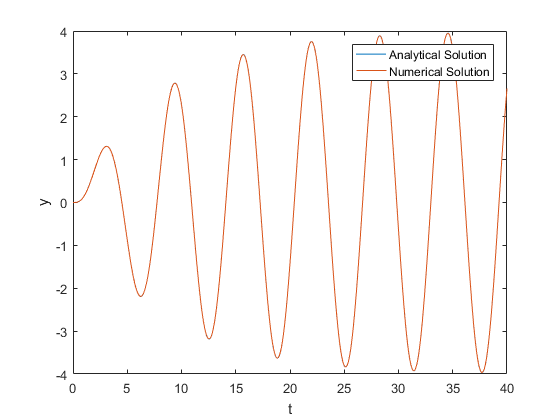
\includegraphics[width=\textwidth]{q7w1g025.png}
\caption{$\omega=1, \gamma=0.25$}
\label{fig:figure1}
\end{minipage}
\hspace{0.5cm}
\begin{minipage}[b]{0.5\linewidth}
\centering
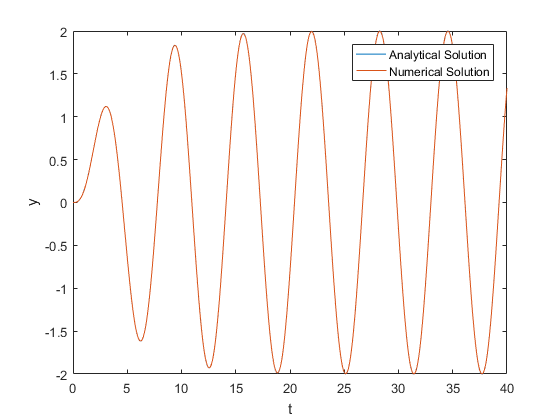
\includegraphics[width=\textwidth]{q7w1g05.png}
\caption{$\omega=1, \gamma=0.5$}
\label{fig:figure2}
\end{minipage}
\end{figure}
	

\begin{figure}[ht]
\begin{minipage}[b]{0.5\linewidth}
\centering
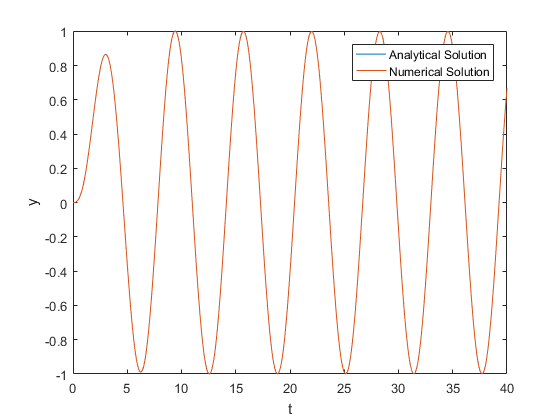
\includegraphics[width=\textwidth]{q7w1g1.png}
\caption{$\omega=1, \gamma=1$}
\label{fig:figure1}
\end{minipage}
\hspace{0.5cm}
\begin{minipage}[b]{0.5\linewidth}
\centering
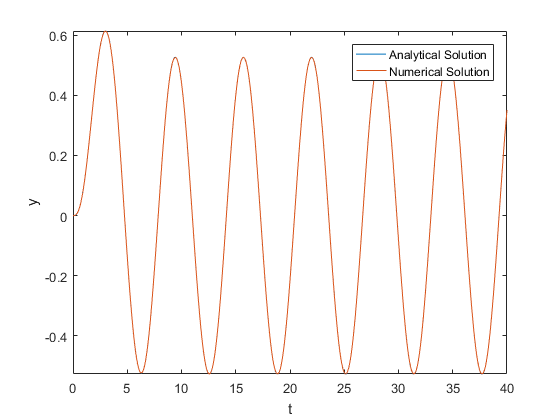
\includegraphics[width=\textwidth]{q7w1g19.png}
\caption{$\omega=1, \gamma=1.9$}
\label{fig:figure2}
\end{minipage}
\end{figure}

\begin{figure}[ht]
\begin{minipage}[b]{0.5\linewidth}
\centering
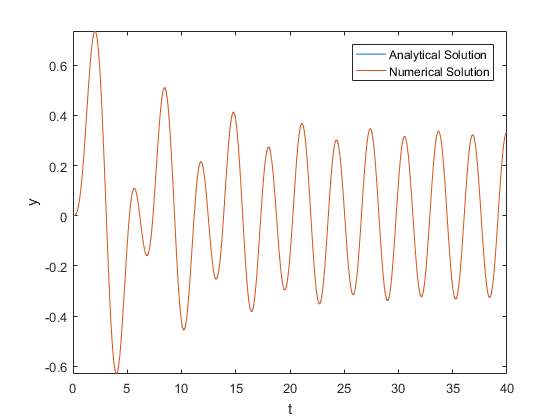
\includegraphics[width=\textwidth]{q7w2g025.png}
\caption{$\omega=2, \gamma=0.25$}
\label{fig:figure1}
\end{minipage}
\hspace{0.5cm}
\begin{minipage}[b]{0.5\linewidth}
\centering
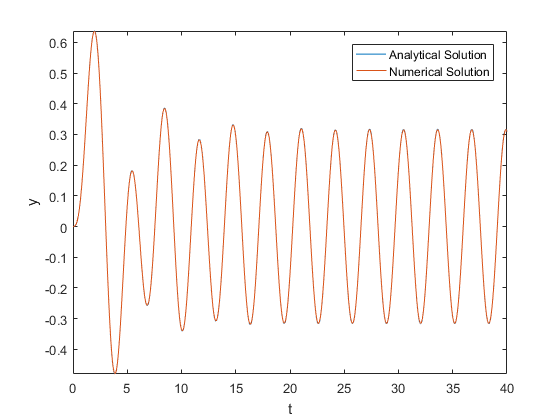
\includegraphics[width=\textwidth]{q7w2g05.png}
\caption{$\omega=2, \gamma=0.5$}
\label{fig:figure2}
\end{minipage}
\end{figure}

\begin{figure}[ht]
\begin{minipage}[b]{0.5\linewidth}
\centering
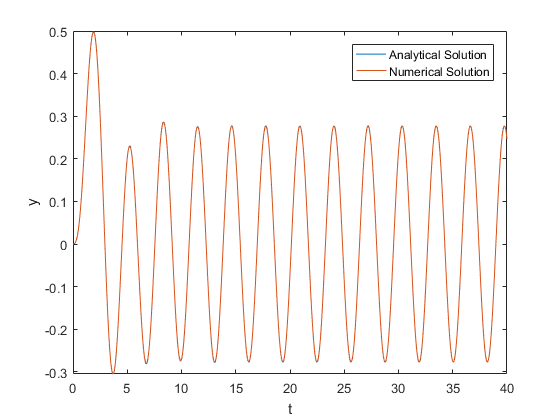
\includegraphics[width=\textwidth]{q7w2g1.png}
\caption{$\omega=2, \gamma=1$}
\label{fig:figure1}
\end{minipage}
\hspace{0.5cm}
\begin{minipage}[b]{0.5\linewidth}
\centering
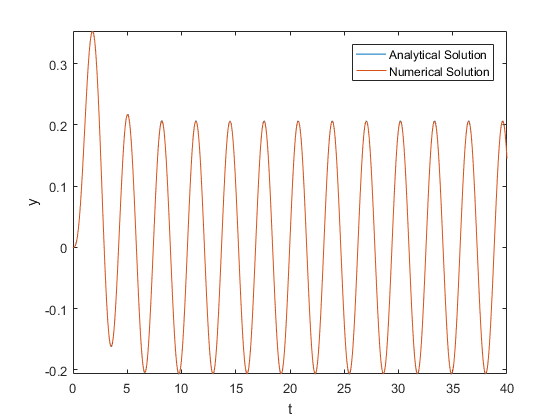
\includegraphics[width=\textwidth]{q7w2g19.png}
\caption{$\omega=2, \gamma=1.9$}
\label{fig:figure2}
\end{minipage}
\end{figure}

\newpage

We start with the obvious features and move on to the more subtle ones after. \par
\vspace{5mm}
Our graphs all seem to approach a sine curve of amplitude $A_s$ as expected from the analytical solution. For fixed $\omega, \Omega$ we see $A_s$ decreases as $\gamma$ increases. In paticular this is a direct inverse proportionality relationship in the case $\omega=1, \Omega=1$ as seen on the graphs.\par
\vspace{5mm}
The difference between $\omega=1$ and $\omega=2$ is a higher frequency and lower amplitude. The amplitude difference can be seen mathematically due to the $A_s$ term, while the frequency changes as the period of the forcing term matches the period of our particular integral, evident mathematically in the $Asin(\omega t-\phi_s)$ form. Physically, consider a system in which there is some restoring force, as well as some damping (as in IA Differential Equations). The system will oscillate at a frequency matching the applied force (if it oscillates at all).\par
\vspace{5mm}
The initial deviation from the sine-like curve is mathematically a result of the the complementary function. For small t, the complementary function is significant, but as t increases its contribution becomes smaller due to the exponential decay. The magnitude of the initial spike depends on both $\gamma$ and $\omega$, with a smaller $\gamma$ producing a larger peak as a result of the form of the coefficients of the complementary function.  Increased $\gamma$ leads to quicker decay to a sine curve due to the $e^{-\frac{\gamma}{2}t}$ in the complementary function. \\

%Note the period of oscillations in the complementary function also $\rightarrow \infty$ as $\gamma\rightarrow 2$.

Physically, we know from IA Differential Equations that $\gamma$ represents some damping (with a scaled time), and increasing $\gamma$ corresponds to  increased damping, removing energy from the system faster, and leading to a quicker decay to steady state. \par

\newpage

\subsection*{Question 8}

Considering the hint, we try to find the first few terms of an series-like 	solution. Considering terms of order $\delta^0$ we get

\begin{equation*}
y_0''(t)+\frac{d}{dt}(\frac{1}{3}\delta^3\delta^{-3}y_{-1}(t)^3)+y_0(t)=sin(t)
\end{equation*}

Substituting the given expressions, expanding as a fourier series, and differentiating the second term we get

\begin{equation*}
-8Csin(3t)-\frac{A^3}{4}sin(t)-\frac{A^3}{4}sin(3t)=sin(t)
\end{equation*}

Equating coefficients of sin(nt) gives $A=-4^{1/3}$ and $C=\frac{1}{8}$. To calculate B, we consider terms of order $\delta$, and get

\begin{equation*}
\delta y_1''(t)+\frac{d}{dt}(\frac{1}{3}3\delta^3\delta^{-2}y_{-1}(t)^2y_0(t))+\delta y_1(t)=0
\end{equation*}

Expanding as a fourier series, and performing the differentiation gives

\begin{equation*}
y_1''(t)+A^2B(\frac{1}{4}cos(t)+\frac{3}{4}cos(3t))+A^2C(\frac{1}{4}cos(t)+\frac{3}{2}cos(3t)+\frac{5}{4}cos(5t)) +y_1(t)=0
\end{equation*}

Since $y_1(t)$ is $2\pi$ periodic, consider its fourier series expansion. Then the coefficient of cos(t) must be 0 on the LHS, giving $A^2B+A^2C=0$ and thus $B=-\frac{1}{8}$. Then we have the approximation, for small $\delta$ 

\begin{equation*}
y=-\delta^{-1}4^{1/3}cos(t)+\frac{1}{8}(sin(3t)-sin(t))
\end{equation*}
	

The script $q8.m$, found on page 20, performs the required task. The graphs are presented below, with the first 2 terms of the series solution superposed. We use h=0.01, unlike question 7, as larger h produced nonsensical graphs, and lowering h any further resulted in unnoticeable differences.

\begin{figure}[ht]
\begin{minipage}[b]{0.5\linewidth}
\centering
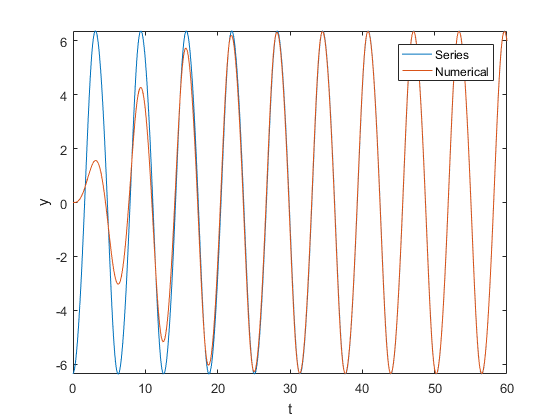
\includegraphics[width=\textwidth]{q8d025.png}
\caption{$\delta=0.25$}
\label{fig:figure1}
\end{minipage}
\hspace{0.5cm}
\begin{minipage}[b]{0.5\linewidth}
\centering
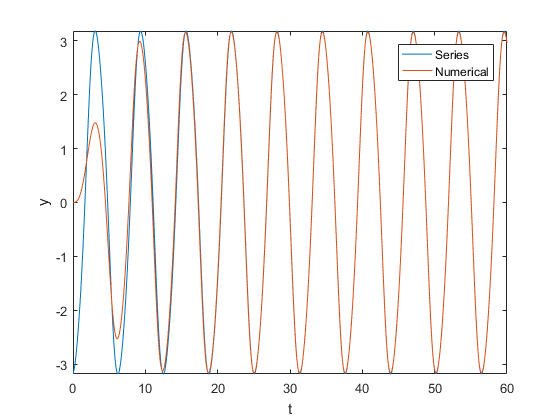
\includegraphics[width=\textwidth]{q8d05.png}
\caption{$\delta=0.5$}
\label{fig:figure2}
\end{minipage}
\end{figure}

\begin{figure}[ht]
\begin{minipage}[b]{0.5\linewidth}
\centering
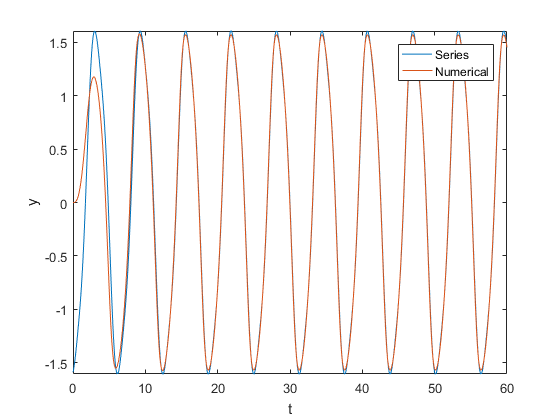
\includegraphics[width=\textwidth]{q8d1.png}
\caption{$\delta=1$}
\label{fig:figure1}
\end{minipage}
\hspace{0.5cm}
\begin{minipage}[b]{0.5\linewidth}
\centering
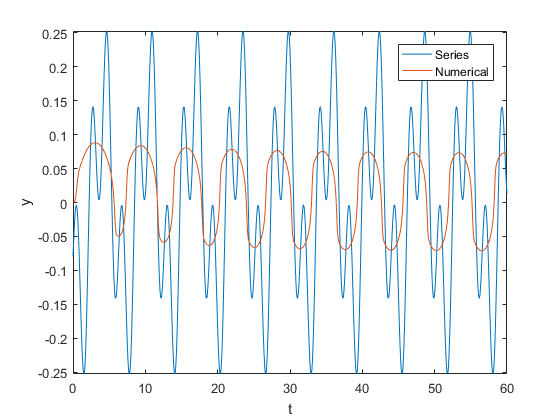
\includegraphics[width=\textwidth]{q8d2.png}
\caption{$\delta=20$}
\label{fig:figure2}
\end{minipage}
\end{figure}

\newpage


Firstly, we see the frequency of all numerical curves is similar, as we should expect since the long term behaviour usually matches the form of the forcing, which is the same sine function in every case. This is why the graphs look very similar to those of question 7, for $\omega=1$. We have a decrease in amplitude of the eventual graph as $\delta$ increases, which can be interpreted physically as an increasing damping, and appears almost exactly inversely proportional. \par
\vspace{0.3cm}
The numerical solution is approximated well by the series solution for large times, for $\delta$ sufficiently small. As $\delta$ is increased, it becomes inaccurate, since the higher order terms we excluded become non negligible. $\delta$ being inversely proportional to the amplitude makes sense here, as the $\delta^{-1}$ term is the dominant term, with the rest being much smaller in magnitude for small $\delta$. The series solution is $2\pi$ periodic however, and doesn't capture the deviation near t=0 from an approximate sine curve.\par
\vspace{0.3cm}
The initial deviation from the sine like curve behaves similarly with changing $\delta$ here as it did in question 7 with changing $\gamma$. It approaches the sine-like curve faster as $\delta$ is increased. This shouldn't be particularly surprising, as both $\delta$ and $\gamma$ are coefficients of $\frac{dy}{dt}$ in the similar ODEs, and hence, physically, increasing both has the effect of an increased damping.




\newpage

\subsection*{Programs}

\vspace{1cm}

\subsubsection*{Comparison of the numerical methods for solving ODEs}

\vspace{0.5cm}

(i) $eulersolve.m$
\begin{verbatim}
function [X,Y] = eulersolve(f,x_0,y_0,h,n)
%implementation of the euler method

Y=[y_0];
X=[x_0];

for i=1:n
    X=[X; X(i)+h];
    Y=[Y;Y(i)+h*f(X(i),Y(i))];
end
\end{verbatim}
\vspace{0.5cm}

(ii) $LFsolve.m$
\begin{verbatim}
function [X,Y] = LFsolve( f,x_0,y_0,h,n )
%we do the first step by euler

X=[x_0;x_0+h];
Y=[y_0; y_0+h*f(x_0,y_0)];

for i=2:n
    X=[X;X(i)+h];
    Y=[Y;Y(i-1)+2*h*f((X(i)),Y(i))];
end

end
\end{verbatim}
\vspace{0.5cm}

(iii) $RK4solveOLD.m$
\begin{verbatim}

function [X,Y] = RK4solve( f,x_0,y_0,h,n )

Y=[y_0]
X=[x_0]

for i=1:n
    
    X=[X; X(i)+h];
    k1=h.*f(X(i),Y(i));
    k2=h.*f(X(i)+h/2,Y(i)+k1/2);
    k3=h.*f(X(i)+h/2,Y(i)+k2/2);
    k4=h.*f(X(i)+h,Y(i)+k3);
    Y=[Y;Y(i)+(k1+2*k2+2*k3+k4)/6];
end

end
\end{verbatim}
\vspace{0.5cm}

(iv) $ProgramTest.m$
\begin{verbatim}
f=@(x,y) exp(x);
anal_y=@(x) exp(x)
y_0=1;
x_0=0;
h=0.5
n=2/h

[X,Ye]=eulersolve(f,x_0,y_0,h,n)
[X,Ylf]=LFsolve(f,x_0,y_0,h,n)
[X,Yrk4]=RK4solve(f,x_0,y_0,h,n)

fplot(anal_y,[0,2])
hold on
plot(X,Ye)
hold on
plot(X,Ylf)
hold on
plot(X,Yrk4)
legend('Analytical Solution','Euler','LF','RK4')
xlabel('x')
ylabel('y')

\end{verbatim}
\vspace{0.5cm}

(v) $q1.m$
\begin{verbatim}
function [X,Y_LF,Y,E] = q1(h)


f=@(x,y) -4*y+3*exp(-x);
anal_y=@(x)exp(-x)-exp(-4*x);
y_0=0;
x_0=0;

n=10/h;

[X,Y_LF]=LFsolve(f,x_0,y_0,h,n)

%constructing the analytical solution at each point
Y=[y_0];
for i=2:n+1
    Y=[Y;anal_y(X(i))];
end

E=Y_LF-Y

%to solve for gamma we have E=exp(gx) log(E)=gx hence g is the gradient of
%a log(absE) x graph - need to remove first line cant log0

Xm = X(2:end);
Em = E(2:end);

p=polyfit(Xm,log(abs(Em)),1)
plot(Xm,log(abs(Em)))
xlabel(p)
ylabel('log(|E|)')

end
\end{verbatim}
\vspace{0.5cm}

(vi) $q3.m$
\begin{verbatim}
f=@(x,y) -4*y+3*exp(-x)
anal_y=@(x)exp(-x)-exp(-4*x)
y_0=0
x_0=0
h=0.4
n=10

[X,Y_E]=eulersolve(f,x_0,y_0,h,n)
[X,Y_RK4]=RK4solve(f,x_0,y_0,h,n)   

fplot(anal_y,[0,4])
hold on
plot(X,Y_E)
hold on
plot(X,Y_RK4)
legend('analytical solution','Euler Solution','RK4 solution')
xlabel('x')
ylabel('y')
\end{verbatim}
\vspace{0.5cm}

(vii) $q4.m$
\begin{verbatim}
f=@(x,y) -4*y+3*exp(-x)
anal_y=@(x)exp(-x)-exp(-4*x)
y_0=0
x_0=0
p=anal_y(0.4)
H=[]
E_E=[]
E_LF=[]
E_RK4=[]

for k=0:17
    n=2^k
    h=0.4/n;     
    H=[H;h];
    

   [X,Y_E]=eulersolve(f,x_0,y_0,h,n);
   [X,Y_LF]=LFsolve(f,x_0,y_0,h,n);
   [X,Y_RK4]=RK4solve(f,x_0,y_0,h,n);
    
   E_E=[E_E;Y_E(n+1)-p];
   E_LF=[E_LF;Y_LF(n+1)-p]
   E_RK4=[E_RK4;Y_RK4(n+1)-p]
end

plot(log(H),log(abs(E_E)))
hold on
plot(log(H),log(abs(E_LF)))
hold on
plot(log(H),log(abs(E_RK4)))
legend('Euler','Leapfrog','RK4')
xlabel('log(h)')
ylabel('log(abs(E))')
\end{verbatim}
\vspace{1cm}

\newpage

\subsubsection*{Numerical solutions of second-order ODEs}

(i) $RK4Solve.m$ which now works for coupled ODE's
\begin{verbatim}
function [X,Y] = RK4solve( f,x_0,y_0,h,n )
%UNTITLED4 Summary of this function goes here
%   Detailed explanation goes here

Y=[y_0]
X=[x_0]

for i=1:n
    
    X=[X; X(i)+h];
    k1=h.*f(X(i),Y(i,:));
    k2=h.*f(X(i)+h/2,Y(i,:)+k1/2);
    k3=h.*f(X(i)+h/2,Y(i,:)+k2/2);
    k4=h.*f(X(i)+h,Y(i,:)+k3);
    Y=[Y;Y(i,:)+(k1+2*k2+2*k3+k4)/6];
end

end
\end{verbatim}
\vspace{0.5cm}

(ii) $ProgramTest2.m$
\begin{verbatim}
f=@(x,y) [y(2),-y(1)];
anal_y=@(x) cos(x)
y_0=[1,0];
x_0=0;
h=1
n=5/h

[X,Y]=RK4solve(f,x_0,y_0,h,n)

fplot(anal_y,[0,5])
hold on
plot(X,Y(:,1))
legend('Analytical Solution','RK4 Solution')
xlabel('x')
ylabel('y')
\end{verbatim}
\vspace{0.5cm}

(iii) $q6.m$
\begin{verbatim}
%Note you must set h in the script beforehand
h=0.1
n=10/h


omega=1 %capital omega
delta=0
gamma=1 
w=sqrt(3) %lower case omega
a=1
t_0=0

y_0=[0,0]

f=@(t,y) [y(2), -gamma*y(2)-delta^(3)*y(1)^2*y(2)-omega^2*y(1)+a*sin(w*t)]


A=w*gamma/(w^2*gamma^2+(w^2-1)^2)
B=(2*w*(w^2-1)+gamma^2*w)/(sqrt(4-gamma^2)*(w^2*gamma^2+(1-w^2)^2))
C=-a*(w^2-omega^2)/(w^2*gamma^2+(w^2-omega^2)^2)
D=-w*gamma*a/(w^2*gamma^2+(w^2-omega^2)^2)
y_anal=@(t)C*sin(w*t)+D*cos(w*t) + exp(-gamma*t/2)*(A*cos(sqrt(4-gamma^2)*t/2)
+B*sin(sqrt(4-gamma^2)*t/2))



[T,Y]=RK4solve(f,t_0,y_0,h,n)


Y_anal=[0]
for i=2:n+1
    Y_anal=[Y_anal; y_anal(T(i))]
end

E=Y(:,1)-Y_anal
\end{verbatim}
\vspace{0.5cm}

(iv) $q7.m$
\begin{verbatim}
%must set gamma and w first
gamma=1.9
w=2

omega=1
delta=0 
a=1
t_0=0

y_0=[0,0]
h=0.1
n=40/h

f=@(t,y) [y(2), -gamma*y(2)-delta^(3)*y(1)^2*y(2)-omega^2*y(1)+a*sin(w*t)]


A=w*gamma/(w^2*gamma^2+(w^2-1)^2)
B=(2*w*(w^2-1)+gamma^2*w)/(sqrt(4-gamma^2)*(w^2*gamma^2+(1-w^2)^2))
C=-a*(w^2-omega^2)/(w^2*gamma^2+(w^2-omega^2)^2)
D=-w*gamma*a/(w^2*gamma^2+(w^2-omega^2)^2)

y_anal=@(t)C*sin(w*t)+D*cos(w*t) + exp(-gamma*t/2)*(A*cos(sqrt(4-gamma^2)*t/2)
+B*sin(sqrt(4-gamma^2)*t/2))


[T,Y]=RK4solve(f,t_0,y_0,h,n)

fplot(y_anal,[0,40])
hold on
plot(T,Y(:,1))
legend('Analytical Solution','Numerical Solution')
xlabel('t')
ylabel('y')
\end{verbatim}
\vspace{0.5cm}

(v) $q8.m$
\begin{verbatim}
%must set delta beforehand
delta=20
omega=1
gamma=0
w=1
a=1
t_0=0
y_0=[0,0]
h=0.01
n=60/h
f=@(t,y) [y(2), -gamma*y(2)-delta^(3)*y(1)^2*y(2)-omega^2*y(1)+a*sin(w*t)]
[T,Y]=RK4solve(f,t_0,y_0,h,n)

A=-4^(1/3)
B=-1/8
C=1/8
y_anal=@(t)delta^(-1)*(A*cos(t))+B*sin(t)+C*sin(3*t)

fplot(y_anal,[0,60])
hold on
plot(T,Y(:,1))
xlabel('t')
ylabel('y')
legend('Series','Numerical')

\end{verbatim}





\end{document}

